\documentclass[Screen16to9,17pt]{foils}
\usepackage{kea-slides}

\usepackage{tabularx}
\usepackage{tikz}
\usetikzlibrary{mindmap,trees}
\usetikzlibrary{shapes.geometric, arrows,automata}
\usetikzlibrary{positioning}

\usepackage{jigsaw}



\tikzset{
    state/.style={
           rectangle,
           rounded corners,
           draw=black, very thick,
           minimum height=2em,
           inner sep=2pt,
           text centered,
           },
}

\externaldocument{siem-log-analysis-exercises}
\selectlanguage{english}


\begin{document}

\mytitlepage
{4. SIEM Visualization and Dashboards}
{KEA Kompetence SIEM and Log Analysis}


\slide{Goals for today}

\hlkimage{6cm}{thomas-galler-hZ3uF1-z2Qc-unsplash.jpg}

Todays goals:
\begin{list2}
\item Visualizations see a lot of examples, knowing possibilities makes it possible to choose
\item Kibana features like importing/exporting dashboards
\item Look at alerting
\end{list2}

Photo by Thomas Galler on Unsplash


\slide{Plan for today}

\begin{list1}
\item Subjects
\begin{list2}
\item Visualizations examples
\item Tool examples
\item Kibana features like importing/exporting dashboards
\end{list2}
\item Exercise theme: Make it easy and pretty
\begin{list2}
\item Importing dashboards
\end{list2}
\end{list1}

\slide{Reading Summary}

\begin{list1}
\item DDS 6. Visualizing Security Data 22
\item DDS 10. Designing Effective Security Dashboards
\item Skim: DDS 11. Building Interactive Security Visualizations
\end{list1}



\slide{Reading Summary, continued}

%\hlkimage{}{}

\begin{quote}
\begin{list2}\small
\item {\bf Data visualizations communicate complexity quickly.} Descriptive statistics (mean, median, variance, and so on) exist to describe and simplify data but tend to remove subtleties that exist. It’s possible to communicate millions of data points in seconds while minimizing the loss of detail and resolution through visualization.
\item {\bf Data visualizations enable recognition of latent patterns.} Patterns that would never be apparent using statistical methods or scanning the data may be revealed through visualization. When data is visually presented, patterns in a single variable or relationships across many variables may leap off the screen.
\item {\bf Data visualizations enable quality control on the data.} Mistakes and errors in data collection or preparation can often be revealed through visualization. Data visualizations can serve as a good and quick sanity check on your work.
\item {\bf Data visualizations can serve as a muse.} It’s been said that most breakthroughs in science didn’t start with a “Eureka!” but instead with a “Huh, that’s odd.” Laying out the data visually can give you a new perspective and help facilitate your thinking and discovery processes.
\end{list2}\end{quote}
Source: DDS 6. Visualizing Security Data

\begin{list2}
\item A light reading chapter, color, eye movements etc.
\end{list2}


\slide{Example plot 6-17 }

\hlkimage{10cm}{jay-service-discovery.png}
Source: DDS 6. Visualizing Security Data

\begin{list2}
\item Interesting graph, and interesting results Changing away from standard ports delay attackers!
\end{list2}


\slide{Reading Summary, continued}

%\hlkimage{}{}

\begin{quote}
  \begin{list2}
  \item {\bf A Dashboard Is Not a Report} ... However, the top-level view should be designed solely to give the viewer situational awareness
  of the desired task.
  \item {\bf A Dashboard Is Not an Art Show}
  \item {\bf Take Care with Colors} - talks about printing, but color blindness is a real problem
  \item {\bf Use Fonts Wisely} - be sure to select one that scales consistently, supports variable width text, and has fixed-width numbers.
  \item {\bf No One Dashboard to Rule Them All} - An iterative process
  \end{list2}
\end{quote}
Source: DDS 10. Designing Effective Security Dashboards

\hskip 2cm
\centerline{\Large Going through dashboards must be part of a procedure}

\slide{Reading Summary, continued}

%\hlkimage{}{}

\begin{quote}
  Getting started with D3 requires only three things—a text editor, the D3 JavaScript library, and
  a web server. To prove this, read through this annotated, basic example of a static bar chart (Figure
  11-11) to see what it’s like to code in D3.
\end{quote}
Source: DDS 11. Building Interactive Security Visualizations

\begin{list2}
\item Skim read chapter!
\item D3.js is fantastic and also fantastically complex, beautiful examples \link{https://d3js.org/}
\item I learned similar things from the NoStarch book, Data Visualization with JavaScript
by Stephen A. Thomas March 2015, 384 pp. ISBN-13: 978-1-59327-605-8 \link{https://nostarch.com/datavisualization}\\
\item Today you can easily start out with Kibana, and defaults
\item Finding recipes for running a full screen Dashboard with a rPi are easy to find
\end{list2}




\slide{Conferences and web sites}

%\hlkimage{}{}

\begin{quote}

\end{quote}

\begin{list2}
  \item Multiple sites and resources are available in this area
  \item FloCon, the international conference on “Using Data to Defend,” \link{https://resources.sei.cmu.edu/news-events/events/flocon/}
  \item Zeek (BroCon) events \link{https://zeek.org/past-events/}
  \item IEEE Symposium on Visualization for Cyber Security, \link{https://vizsec.org/}
  \item Secviz older web site I have browsed from time to time, seeing examples, tools, data
  \link{https://secviz.org/}
  \item Greg Conti \link{http://rumint.org/}
\item List a couple of tools you should know by name at least
\item graphviz \link{https://graphviz.org/}
\item afterglow \link{http://afterglow.sourceforge.net/}, examples Raffael Marty
\link{https://raffy.ch/blog/2012/03/24/advanced-network-graph-visualization-with-afterglow/}
\end{list2}

\centerline{Take names, make a list - note the tools and people working with this}

\slide{Newer tools}

% \hlkimage{2cm}{seaborn_scatterplot_sizes_thumb.png}

\begin{list2}
  \item \link{https://www.brimsecurity.com/} Brim now renamed Zui is packaged as a desktop app, built with Electron just like Slack. Once installed, you can open a pcap with Zui and it will transform the pcap into Zeek logs in the ZNG format.
  \item \link{https://seaborn.pydata.org/} Seaborn is a Python data visualization library based on matplotlib. It provides a high-level interface for drawing attractive and informative statistical graphics.
  \item \link{https://www.scikit-yb.org/en/latest/}  Yellowbrick extends the Scikit-Learn API to make model selection and hyperparameter tuning easier. Under the hood, it’s using Matplotlib.
  \item \link{https://altair-viz.github.io/} Altair is a declarative statistical visualization library for Python, based on Vega and Vega-Lite, and the source is available on GitHub.
  \item \link{https://github.com/gtkcyber/griffon-vm} Griffon is a environment for data science. Griffon is based on Ubuntu MATE and includes numerous data science tools, all installed and configured for immediate use.
\end{list2}

Recommended by Charles Givre in the article:\\
\link{https://www.oreilly.com/content/improving-security-through-data-analysis-and-visualizations/}


\slide{Books: Network Security Through Data Analysis}

\hlkimage{3cm}{network-security-through-data-analysis.png}

Network Security through Data Analysis, 2nd Edition
By Michael S Collins
Publisher: O'Reilly Media
2015-05-01: Second release, 348 Pages

\begin{list2}
\item \emph{Applied security visualization}, Rafael Marty, 2009
\item \emph{Security Data Visualization: Graphical Techniques for Network Analysis}, Greg Conti 2007
\item \emph{Visualize This: The FlowingData Guide to Design, Visualization, and Statistics}, Nathan Yau
ISBN: 978-0-470-94488-2 July 2011 384 Pages
\end{list2}


\slide{Example tools and graphs}

\hlkimage{12cm}{etherape-2018.png}


\begin{list2}
  \item Graph types not in the book
  \item Etherape shown, see \url{https://etherape.sourceforge.io/}
\end{list2}


\slide{Parallel coordinate plots}

\hlkimage{16cm}{collberg-parallel-plot.png}
Source: image from Network Security Visualization Keith Fligg and Genevieve Max\\
\link{https://www2.cs.arizona.edu/~collberg/Teaching/466-566/2013/Resources/presentations/2012/topic13-final/report.pdf}

\begin{list2}
\item \link{https://en.wikipedia.org/wiki/Parallel_coordinates}
\item Nice for explaining connections, but not used much in real life systems
\end{list2}





\slide{Hosting and internet providers}

\hlkimage{16cm}{network-bgp-asn.png}

\begin{list2}
\item BGP networks are used for all of the Internet
\item New standards like Resource Public Key Infrastructure (RPKI) are underway
\item Try RIPE BGPlay \url{https://stat.ripe.net/special/bgplay#bgplay_fetch.resource=185.129.60.1}
\end{list2}



\slide{Monitor your network}

\begin{slidelist}
\item MRTG The Multi Router Traffic Grapher - simple, great, fast\\
\link{http://oss.oetiker.ch/mrtg/}
\item Smokeping Network Latency measurements - network quality\\
 \link{http://oss.oetiker.ch/smokeping/}
\item NFsen Netflow monitoring - turn on at selected routers/switches
\item LibreNMS \link{https://www.librenms.org/}
\item Manual tools, My Traceroute, Nping
\end{slidelist}

\slide{MRTG SNMP monitoring made easy}

\hlkimage{13cm}{images/mrtg-small.png}

\centerline{Run configmaker, indexmaker - almost done}

\slide{Smokeping packet loss}

\hlkimage{12cm}{images/smokeping-packet-loss1}

\slide{Smokeping latency changed}

\hlkimage{12cm}{images/smokeping-latency-change.png}


\slide{Autoconfiguration: location}

\hlkimage{16cm}{images/snmp-location.png}

\centerline{Observium picks up the location from SNMP :-)}

\slide{Config example: LLDP}
%\hlkrightimage{8cm}{images/lldp-dell-8024f.png}

Dell 8024F switch LLDP
\hlkrightpic{10cm}{0cm}{images/lldp-dell-8024f.png}


\begin{alltt}\small
interface ethernet 1/xg17
mtu 9216
lldp transmit-tlv port-desc sys-name sys-desc sys-cap
lldp transmit-mgmt
exit
\end{alltt}

\slide{Autoconfigured maps from LLDP}
\hlkimage{\textwidth-3cm}{images/lldp-mess-censor.png}

\centerline{LLDP is needed!}

\slide{Netflow processing from the web interface}

\hlkimage{12cm}{images/nfsen-processing-1.png}

\centerline{Bringing the power of the command line forward}

\slide{LibreNMS Automatic discovery}

\hlkimage{10cm}{librenms-switches.png}

Automatically discover your entire network using CDP, FDP, LLDP, OSPF, BGP, SNMP and ARP.

\slide{LibreNMS Geo Location}
\hlkimage{12cm}{librenms-geo-location.png}

\slide{LibreNMS wireless clients}
\hlkimage{20cm}{images/librenms-wireless-clients.png}


\slide{Demo}

%\hlkimage{}{}

\begin{quote}

\end{quote}

\begin{list2}
  \item Demo: Unifi dashboard
  \item Demo: LibreNMS and Smokeping
\end{list2}


\slide{Before testing: Pingdom}

\hlkimage{18cm}{forside-pingdom.png}

\centerline{Another external monitoring from Pingdom.com}

\slide{Problems in the network}



\hlkimage{20cm}{smokeping-3.png}

\centerline{Oh no DDoS attack?}


\slide{What to put into the Dashboard}


Chapter 11. Anomaly-Based Detection with Statistical Data

Good advice found in the book:
\begin{list2}
\item Top Talkers with SiLK
\item Service Discovery with SiLK
\item Furthering Detection with Statistics
\item Visualizing Statistics with Gnuplot
\item Visualizing Statistics with Google Charts
\item Visualizing Statistics with Afterglow
\end{list2}

Newer and other tools exist, but the process is the same.

Source: Applied Network Security Monitoring Collection, Detection, and Analysis, 2014 Chris Sanders ISBN: 9780124172081

\slide{Map sources to dashboards!}

%\hlkimage{}{}


\begin{center}
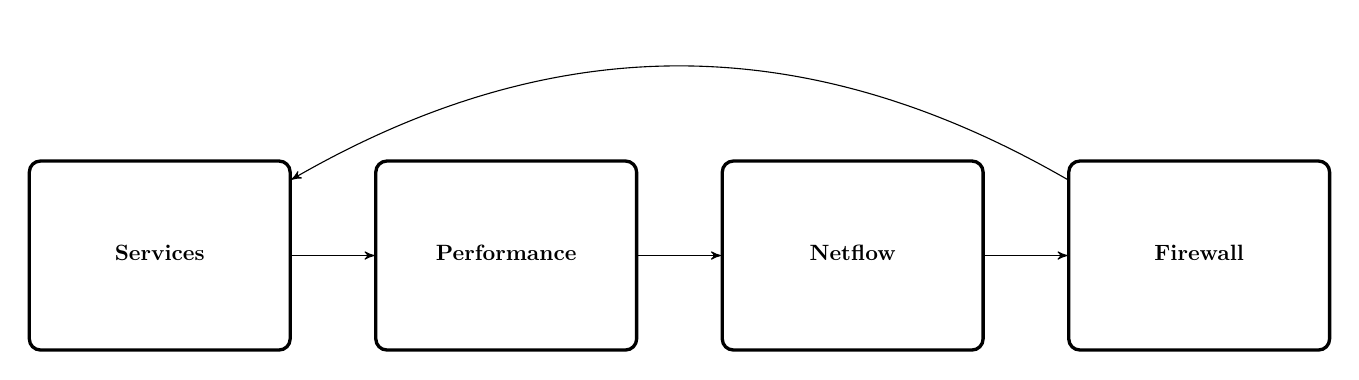
\begin{tikzpicture}[->,>=stealth',scale=0.8, transform shape]
  \newlength{\boxwidth}
  \newlength{\boxheight}
  \newlength{\boxspace}
  \setlength{\boxwidth}{4cm}
  \setlength{\boxheight}{3cm}
  \setlength{\boxspace}{55mm}

  % http://texample.net/tikz/examples/epc-flow-charts/

  % https://www.overleaf.com/learn/latex/LaTeX_Graphics_using_TikZ:_A_Tutorial_for_Beginners_(Part_3)%E2%80%94Creating_Flowcharts

   % Use previously defined 'state' as layout (see above)
   % use tabular for content to get columns/rows
   % parbox to limit width of the listing
   \node[state,text width=\boxwidth,minimum height=\boxheight] (SERVICES)
   {\begin{tabular}{l}
   {\bf Services}
   \end{tabular}};
   %
   \node[state,         % layout (defined above)
    text width=\boxwidth,       % max text width
    minimum height=\boxheight,
    %yshift=2cm,                % move 2cm in y
    right of=SERVICES,    % Position is to the right of QUERY
    node distance=\boxspace,    % distance to First node
    anchor=center] (PERFORMANCE)   % posistion relative to the center of the 'box'
    {\begin{tabular}{l}
    {\bf Performance}
    \end{tabular}};

    \node[state,         % layout (defined above)
     text width=\boxwidth,       % max text width
     minimum height=\boxheight,
     %yshift=2cm,                % move 2cm in y
     right of=PERFORMANCE,    % Position is to the right of QUERY
     node distance=\boxspace,    % distance to First node
     anchor=center] (NETFLOW)   % posistion relative to the center of the 'box'
     {\begin{tabular}{l}
     {\bf Netflow}
     \end{tabular}};

     \node[state,         % layout (defined above)
      text width=\boxwidth,       % max text width
      minimum height=\boxheight,
      %yshift=2cm,                % move 2cm in y
      right of=NETFLOW,    % Position is to the right of QUERY
      node distance=\boxspace,    % distance to First node
      anchor=center] (FIREWALL)   % posistion relative to the center of the 'box'
      {\begin{tabular}{l}
      {\bf Firewall}
      \end{tabular}};


   % draw the paths and and print some Text below/above the graph
   \path
   (SERVICES) edge (PERFORMANCE)
   (PERFORMANCE) edge (NETFLOW)
   (NETFLOW) edge (FIREWALL)
   (FIREWALL) edge[bend right] (SERVICES)
   ;
\end{tikzpicture}
\end{center}


\begin{list2}
\item There are many input sources available
\item Dont put them all in ONE DASHBOARD
\item I had luck in creating multiple dashboards, and then having a display cycle through them
\item Maybe use Elastic Spaces for this? \link{https://www.elastic.co/guide/en/kibana/master/xpack-spaces.html}
\end{list2}


\slide{Applied Security Visualization examples}


\hlkimage{13cm}{applied-security-visualization-firewall.png}

Source: Firewall Report in \emph{Applied security visualization}, Rafael Marty, 2009

\slide{Applied Security Visualization examples}


\hlkimage{10cm}{applied-security-visualization-flow.png}

Source: Network Flow Data in \emph{Applied security visualization}, Rafael Marty, 2009



\slide{Drill down process}

%\hlkimage{}{}

\begin{quote}

\end{quote}

\begin{enumerate}
\item Get an overview
\item Research top talkers,
\item When identified and handled, remove with filter \verb+not host 10.1.2.3+
\item Look at the next ones
\end{enumerate}

Look into details, lookup hostnames -- hopefully your tool allows some help



\slide{Alerting}

%\hlkimage{}{}

\begin{quote}\small
We’re excited to announce a new alerting framework that delivers a first-class alerting experience natively within the SIEM, Uptime, APM, and Metrics applications as part of the Kibana 7.7 release.

Alerting is a fundamental use case across the Elastic Stack, which is why we’re making it part of the core experience within Kibana. Whether you are monitoring application transactions or tracking brute force login attempts, our goal is to provide a tailored experience that allows you to build powerful alerts in the normal flow of your task. The new alerting framework is built from the ground up and designed to offer more than just convenient interfaces. We understand the need to go beyond just notifying people which is why we’ve also incorporated the ability to trigger predefined actions that can do anything from sending an email to using brand new third-party integrations with platforms like Slack and PagerDuty.

The new alerting framework is being introduced as a beta in the 7.7 release of Kibana and is available immediately on the Elasticsearch Service on Elastic Cloud, or for download.
\end{quote}

\begin{list2}
\item\link{https://www.elastic.co/blog/introducing-the-new-alerting-framework-for-observability-security-and-the-elastic-stack}
\item \link{https://www.elastic.co/what-is/kibana-alerting}
\item \link{https://www.elastic.co/blog/alerting-in-the-elastic-stack}
\item \link{https://www.elastic.co/blog/elastic-stack-alerting-now-generally-available}
\end{list2}


\slide{Alerting everywhere}

%\hlkimage{}{}

\begin{quote}
Alerting everywhere: Kibana 7.7 introduces ubiquitous alerting for Elastic Observability, Elastic Security, and the Elastic Stack. Users can now create alerts directly from within the SIEM, APM, Metrics, and Uptime applications as well as for any index.
\end{quote}

\begin{list2}
\item Seems a lot has happened with alerting in the new version!
\item Lets try to work with the alerting framework, note: sending email can sometimes be tricky without some configuration.
\end{list2}

\exercise{ex:kibana-kts}

\slide{Reporting}

\centerline{\bf\Large Moving to next time, with baseline your data}

Discussion! Writing and presenting are two very different things, so are dashboards and reports!

\slidenext{}


\end{document}
